\section{Augmenting SLAM with Wi-Fi Sensing}
\label{sec:soln}
To demonstrate the utility of augmenting visual SLAM with Wi-Fi, we instrument three well-known SLAM algorithms with Wi-Fi sensing. For this, we chose RGBD SLAM~\cite{burgard:rgbd-slam}, RTAB-Map~\cite{rtabmap} and ORB-SLAM~\cite{orbslam}. All of them have open-source implementations making it convenient to modify them. In RGBD SLAM and ORB-SLAM, no odometry information is used which makes them easy to use on wearable devices as well as robots. We now describe each instrumentation in detail. For this, we first describe the original SLAM system followed by a description of our augmentation. 
\subsection{RGBD SLAM}
\subsubsection{\textbf{Background}}
RGBD SLAM~\cite{burgard:rgbd-slam} is a graph-based visual SLAM where nodes correspond to RGBD frames and edges correspond to 3D visual transformations between them. Also, any frame with unique visual features constitutes a keyframe.
RGBD SLAM represents an early SLAM system built for RGB-D sensors. It is somewhat brittle and computationally heavy as shown in our results.

Figure~\ref{fig:RGBD_box} shows a block diagram of RGBD SLAM. We also show how Wi-Fi sensing is augmented in red using the described modules in general proposed approach. 
In RGBD SLAM, each new frame is compared to a subset of previous frames for motion estimation and place recognition (Node Selection in Figure~\ref{fig:RGBD_box}). 
(a) {\it Predecessor Nodes}: A fixed number of nodes prior to the current node, (b) {\it Geodesic Neighbors}: A fixed depth of the graph before the current node, and (c) {\it Keyframes}: A randomized sub-set of previous keyframes. Intuitively, the predecessor nodes and geodesic nodes are used for motion estimation and the random sub-set of keyframes are for identifying long-term loop closures. Ideally, each frame should be compared with all relevant keyframes for best results. 
However, this is not tractable since the number of keyframes increases as the map grows. 
Thus, the keyframe selection is limited to a constant random number to reduce the computational complexity of this step as the map grows. This results in lower probability of finding correct long-term loop closures over time as the size of the graph increases.

\begin{figure}
%\vspace{-20pt}
\centering
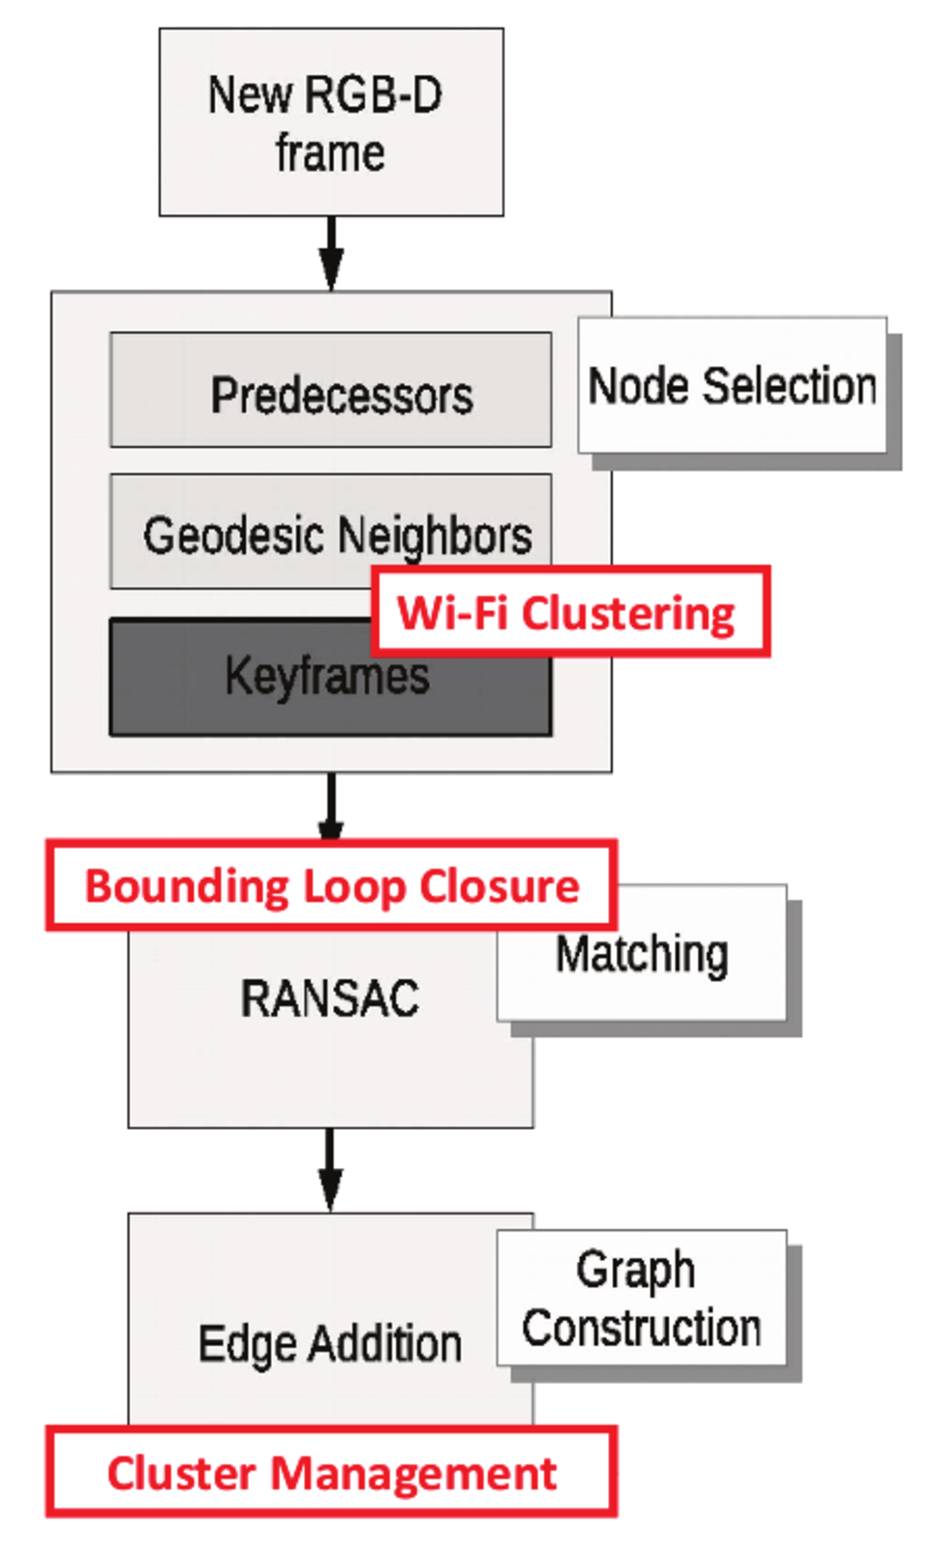
\includegraphics[width=0.2\textwidth]{Figure3.eps}
\caption{Control Flow of RGBD SLAM for each new RGBD frame. Our augmentation of Wi-Fi sensing is shown in red}
\label{fig:RGBD_box}
\vspace{-15pt}
\end{figure}

\subsubsection{\textbf{Wi-Fi Augmentation}}
We intend to improve long-term loop closure (avoiding perceptual aliasing) by incorporating Wi-Fi sensing. As discussed earlier, %choosing a random set of keyframes results in poor loop closure detection and 
comparing all keyframes to the current frame results in huge computational overhead. It would be ideal to select a subgraph of the existing map that corresponds to the places close (distance-wise) to current frame for loop closure. This should improve the accuracy of loop closure detection along with runtime reduction. %while not increasing the computational complexity significantly. 

To improve the selection of related keyframes, we apply our proposed approach.
\begin{itemize}
\item \textbf{Wi-Fi Clustering:} We divide the RGBD keyframes into different clusters based on their Wi-Fi signature. 
For each new RGBD frame, we compute the cosine similarity between its signature and the representative signatures of all clusters to find {similar clusters}. 
\item \textbf{Bounding Loop Closure Search:} We compare the current frame only to RGBD keyframes within {similar clusters} for visual transformation calculation.
This approach limits the number of keyframes to be compared against for loop closure detection. 
\item \textbf{Cluster Management:} If the current frame is identified as an RGBD keyframe, this module is activated for assigning it to the right cluster as discussed in~\ref{sec:slam}.
\end{itemize}
Keyframe clustering based on the similarity between Wi-Fi signatures allows us to select a subset of RGBD keyframes that correspond to the similar location range as the current frame for loop closure detection. Also, due to low computation overhead of determining Wi-Fi similarity, we can compute similarities between the current Wi-Fi signature and {\it all} Wi-Fi clusters quickly, which is very beneficial in identifying keyframes from close-by regions from the whole map instead of picking random keyframes like the original method. This allows us to not only improve the loop closure accuracy but also decrease computational complexity. 

\subsection{RTAB-Map}
\subsubsection{\textbf{Background}}
RTAB-Map~\cite{rtabmap} is a real-time graph-based method similar to RGBD SLAM in structure, but it uses odometry. This makes it particularly suitable for robots or wearable devices with inertial sensing and low mobility. The main difference between RTAB-Map and RGBD SLAM is the way memory is managed and loop closure detection is handled.

In this algorithm, three types of memories are defined; Short Term Memory(STM), Working Memory(WM) and Long-Term Memory.
(a) STM is for a fixed number of the most recently added nodes %which would act as predecessor nodes for current node
, (b) WM includes the nodes which are candidates for comparison for loop closure detection. Every node is transferred from STM to WM after a while, and 
 (c) LTM is for the nodes which will not be used for any purpose anytime soon. 
 Figure~\ref{fig:RTABMAP_flowchart} shows the different memories and their interactions along with segments with our augmentation in red. We have built two additional modules called {\it Wi-Fi Immunization} and {\it Wi-Fi Cluster Retrieval} which are specific to this algorithm apart from those in our general approach. 
\begin{figure}
\centering
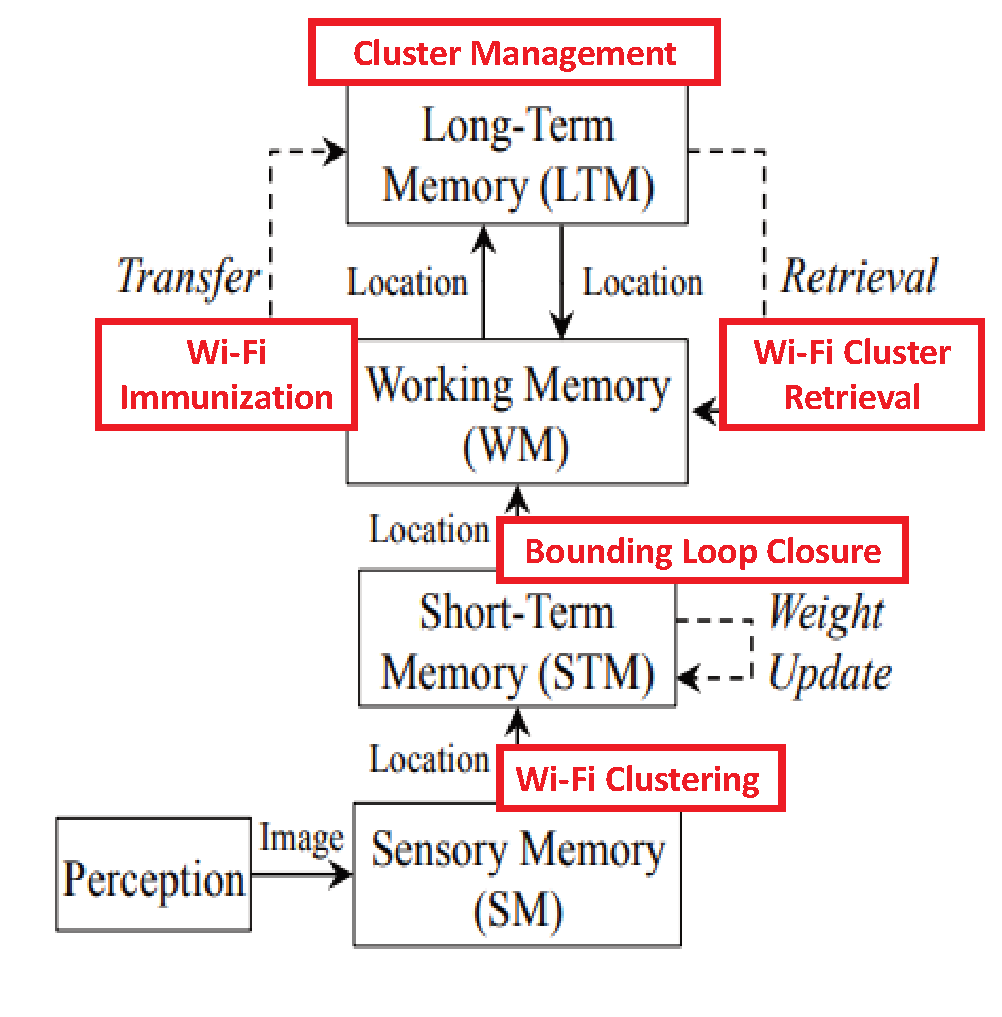
\includegraphics[width=0.3\textwidth]{Figure4.eps}
    \caption{Block diagram of the workflow of RTAB-Map for each new RGBD frame~\cite{rtabmap} along with our Wi-Fi sensing augmentation in red.}
\label{fig:RTABMAP_flowchart}
\vspace{-20pt}
\end{figure}

One of the parameters that a user can control in the RTAB-Map system is {\tt real\_time threshold}. This corresponds to the time that is considered acceptable for the processing of a new frame. During the execution, whenever the processing time of the current node exceeds the specified {\tt real\_time threshold}, some nodes are transferred from WM to LTM. Selection of nodes for transfer is done based on many criteria such as nodes that are not graph-wise close (i) to the current node and (ii) to nodes which have high visual similarity with the current node. While these conditions are reasonable, there is still a fair chance of losing relevant candidates, especially for long-term loop closure as discussed in the original paper~\cite{rtabmap}.
\subsubsection{\textbf{Wi-Fi Augmentation}}
RTAB-Map trades off localization and mapping accuracy for computational efficiency by moving frames from working memory (WM) to long-term memory (LTM). This process increases the probability of missing a loop closure due to unavailability of related frames in WM. We intend to improve the choice of frames to transfer to LTM using Wi-Fi sensing. 
\begin{itemize}
\item \textbf{Wi-Fi Clustering:} Upon arrival of a new frame, we compute the cosine similarity between the new Wi-Fi signature and all Wi-Fi clusters within memory in order to find {similar clusters}. 
\item \textbf{Wi-Fi Immunization:} If the RGBD frames of {similar clusters} are in WM, they are marked not to be moved to LTM. 
\item \textbf{Wi-Fi Cluster Retrieval:} If the RGBD frames of {similar clusters} are in LTM, they are retrieved back to WM and marked not to be moved to LTM.
\item \textbf{Bounding Loop Closure Search:} Visual transformation calculation happens between the current frame and the frames within {similar clusters}.
\item \textbf{Cluster Management:} The current frame is assigned to the right Wi-Fi cluster as discussed in~\ref{sec:slam}.
\end{itemize}  
\subsection{ORB-SLAM}
\subsubsection{\textbf{Background}}
ORB-SLAM is a recent graph-based visual SLAM algorithm similar to RGBD SLAM in structure. A primary contribution of this algorithm is the construction of a dictionary relating visual words to keyframes which have observed them. This dictionary helps in quick lookup of similar keyframes (ones with similar visual words) for comparison to current keyframe for long-term loop closure. In this manner, each new keyframe is compared to the keyframes which have at least one visual word in common with it.
Another contribution is the definition of co-visible keyframes which identifies keyframes sharing map points. Figure~\ref{fig:orbslam_flowchart} shows the block diagram of ORB-SLAM along with segments where Wi-Fi modules are incorporated in red. 
Although the dictionary lookup approach increases the probability of accurate detection of positive loop closures, it still suffers from perceptual aliasing in symmetric environments.
\begin{figure}
%\vspace{-20pt}
\centering
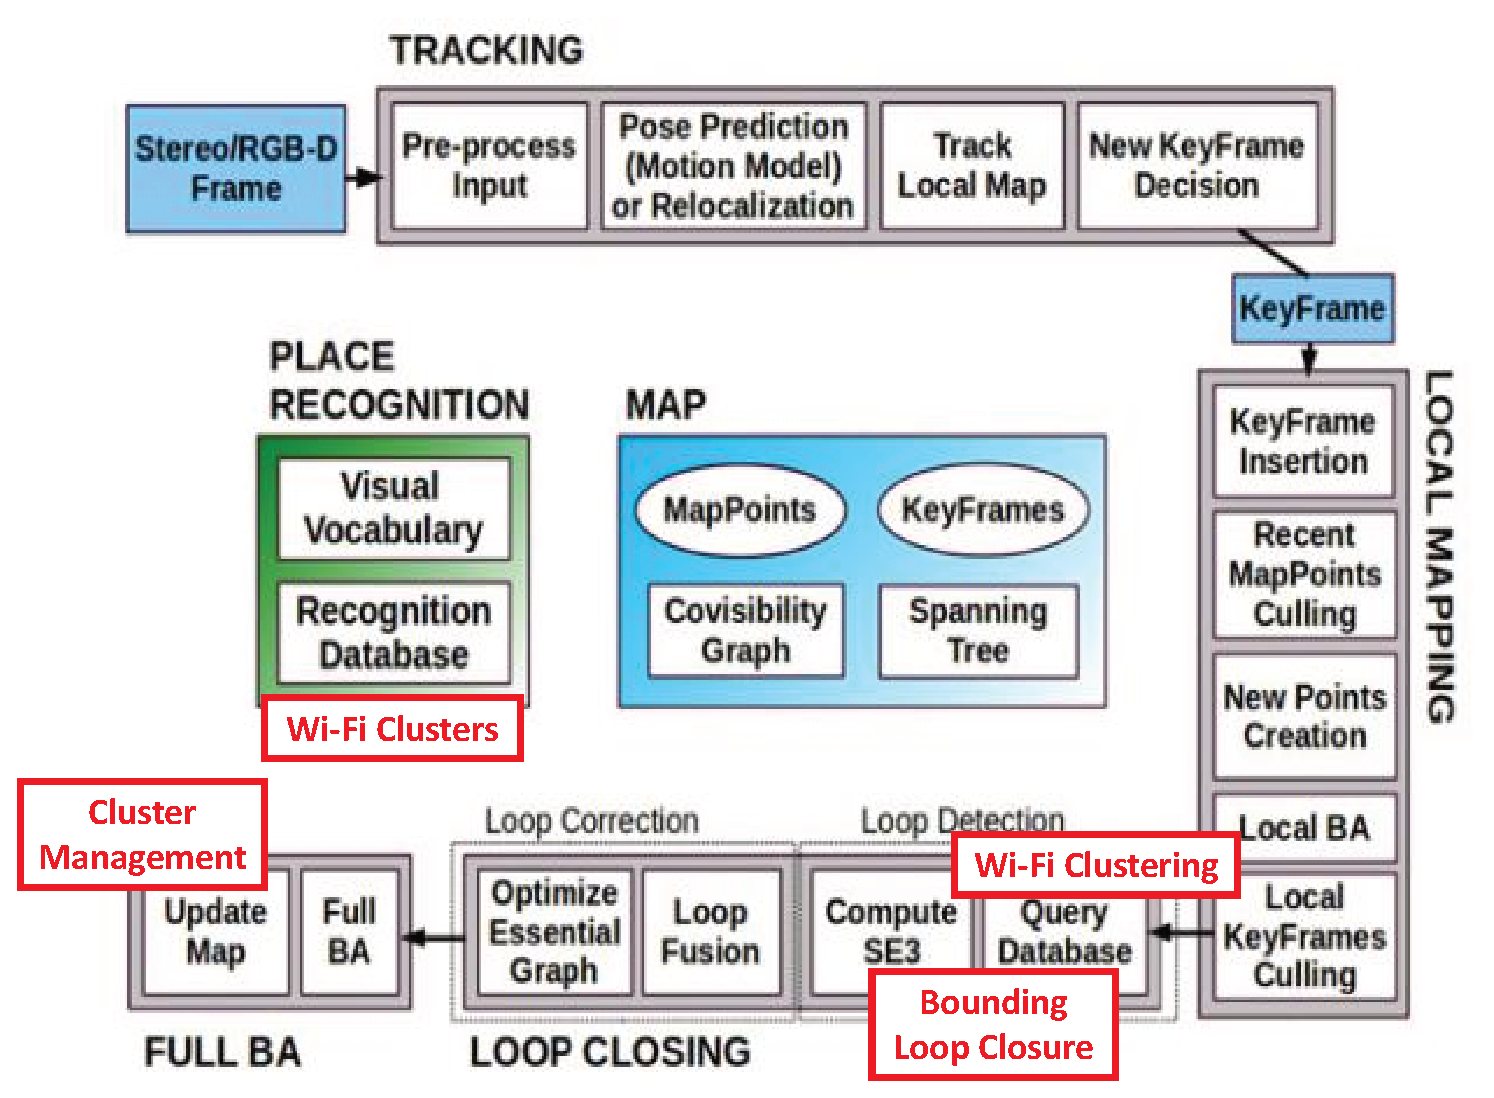
\includegraphics[width=0.45\textwidth]{Figure5.eps}
    \caption{Control flow of ORB-SLAM for each new RGBD frame~\cite{orbslam} along with our incorporation of Wi-Fi sensing in red.}
\label{fig:orbslam_flowchart}
\vspace{-15pt}
\end{figure}
\subsubsection{\textbf{Wi-Fi Augmentation}}
In ORB-SLAM, there is a visual word dictionary which maps visual words to RGBD keyframes which have observed them. For loop closure detection, each RGBD keyframe is compared to any keyframe which has at least one common visual word with it. While this approach probably would be able to find any correct loop closure, it is not immune to perceptual aliasing. Incorporating Wi-Fi sensing could alleviate this problem. Here is how we augment ORB SLAM with Wi-Fi sensing.
\begin{itemize}
\item \textbf{Wi-Fi Clustering:} We compute the cosine similarity between the Wi-Fi signature of new RGBD keyframe to all available Wi-Fi clusters to find {similar clusters}. 
\item \textbf{Bounding Loop Closure Search:} We only use the visual word dictionaries of {similar clusters} for finding RGBD keyframes which have visual words in common with the current frame. This would significantly lower the number of candidates for comparison and reduce the chances of perceptual aliasing.
\item \textbf{Cluster Management:} If a valid visual edge is constructed or there are any co-visible keyframes within {similar clusters}, the current frame is assigned to the corresponding cluster. Otherwise, a new Wi-Fi cluster with a separate visual word dictionary is created.
\end{itemize} 
We intend to open-source all implementations that we have augmented with Wi-Fi sensing on the publication of this work. We hope that this will help the community refine integrating Wi-Fi sensing and visual sensing. We will now evaluate the performance of each of our Wi-Fi augmented SLAM systems and compare them to the original approaches. 
